\documentclass[12pt, a4paper, twoside, openright]{book}

\usepackage[french]{babel}
\usepackage[T1]{fontenc}
\usepackage[utf8]{inputenc}
\usepackage{lmodern}
\usepackage{graphicx}
\usepackage{hyperref}
\usepackage{listings}
\usepackage{graphicx}
\usepackage{microtype}
\usepackage{glossaries}
\usepackage{color}
\makeglossaries %à la suite de la déclaration de package
\newglossaryentry{table}
        {name={table},
        plural={tables},
        description={Ensemble d'\textit{attributs}.
        dans une base de données relationnelle, chaque ligne d'une table (nommée \textit{tuple}) est identifiée
        par un attribut ou groupe d'attributs
        uniques dans la table, que l'on nomme \textit{clée primaire}.
        Pour simplifier, on peut voir les tables comme des tableaux à une entrée : le nombre de colonnes est fixé, en revanche le nombre de lignes ne l'est pas. La figure \ref{exemple_table} représente une table}}

\newglossaryentry{tuple}
        {name={tuple},
        plural={tuples},
        description={Une \textit{ligne} de données dans une table. Une table contient de 0 à n tuples}}
        
        
\newglossaryentry{JDBC}
{
  name=JDBC,
  description={Java DataBase Connectivity est une interface de programmation permettant de manipuler des bases de données avec des objets. Les systèmes de gestion de base de données doivent fournir un pilote JDBC correspondant à l'implémentation de cette interface}
}

\newglossaryentry{JRE}
{
  name=JRE,
  description={Java Runtime Environment correspond à l'environnement d'exécution d'une application Java. Cet environnement est composé d'une machine virtuelle chargée d'exécuter les fichiers compilées ainsi que des bibliothèques standards fournies par Java}
}

\newglossaryentry{MVC}
{
  name=MVC,
  description={Modèle-Vue-Contrôleur est une façon d'organiser le code de programmation qui est optimale pour les logiciels ayant une interface graphique}
}

\newglossaryentry{commit}
{
  name=commit,
  description={Instruction demandant au SGBD de valider sur la base de données toutes les actions préalablement mises en "cache". Les modifications effectuées deviennent visibles pour les autres utilisateurs du SGBD}
}

\newglossaryentry{attribut}
        {name={attribut},
        plural={attributs},
        description={Un nom de colonne dans une table, également appelé \textit{champ}.
        Une table contient au moins un attribut}}
        
\newglossaryentry{data}{
        name={donnée},
        plural={données},
        description={Valeur brute, sans signification si aucun contexte n'est disponible. Du croisement des données résulte de l'information}}

\newglossaryentry{bdd}{
        name={base de données},
        plural={bases de données},
        description={Abrégé \textit{BD}. Outil permettant de stocker et de retrouver des ensembles des données.
        Dans ce rapport, ne sont mentionnées que des bases de données informatisées et relationelles}}

\newglossaryentry{bddr}{
        name={base de données relationnelle},
        plural={bases de données relationnelles},
        description={Abrégé \textit{BDR}. Il existe plusieurs types de bases de données.
        Dans ce rapport, ne sont mentionnées que des bases de données \textit{relationnelles}.
        Les données sont stockées dans des \textit{tables}, et les tables sont reliées entre elles par leurs clées primaires}}
        
        
\newacronym[plural={LDD},
        first={Langage de Définition des Données (LDD)},
        firstplural={Langages de Définition des Données}]
        {ldd}
        {LDD}
        {Langage de Définition des Données, un sous-ensemble du langage SQL permettant de décrire la structure des tables et les relations entre elles. Très grossièrement, le LDD permet de définir les tables et leurs colonnes}

\newacronym[plural={LMD},
        first={Langage de Manipulation des Données (LMD)},
        firstplural={Langages de Manipulation des données}]
        {lmd}
        {LMD}
        {Langage de Manipulation des Données, un sous-ensemble du SQL permettant d'effectuer les opérations CRUD sur les données contenues dans les tables}

\newacronym[plural={SQL},
        first={Structured Query Language (SQL)}]
        {sql}
        {SQL}
        {Structured Query Langage, un langage déclaratif et normé permettant d'utiliser les bases de données relationelles, largement inspiré par Codd en 1970 et devenu un standart aux Etats-Unis en 1984}

\newacronym[first={Create, Read, Update, Delete (CRUD)}]
                           {crud}
                           {CRUD}
                           {Create, Read, Update, Delete sont les quatre opérations basiques à effectuer sur des enregistrements de données, respectivement : en ajouter des nouveaux, les lire, les mettre à jour et les effacer}

\newacronym[first={système d'Information (SI)},
                           firstplural={Systèmes d'Information (SI)}]
                           {si}
                           {SI}
                           {Le Système d'Information est un ensemble organisé de ressources qui permet de collecter, stocker, traiter et distribuer de l'information}

\newacronym[first={Système de Gestion de Base de Données (SGBD)},
                           firstplural={Systèmes de Gestion de Base de Données (SGBD)},
                           plural={SGBD}]
                           {sgbd}
                           {SGBD}
                           {Système de Gestion de Base de Données, logiciel permettant la définition et la manipulation des bases de données. Dans ce rapport, ne sont mentionnés que des logiciels agissant sur des bases de données relationnelles}

\newglossaryentry{query}
        {name={requête SQL},
        plural={requêtes SQL},
        description={Une requête SQL est le nom couramment associé à du code SQL fonctionnel qui interroge ou agit sur la base de données}}

\newacronym[first={Interface Homme-Machine (IHM)},
	firstplural={Interfaces Homme-Machine (IHM)},
        plural={IHM}]
	{ihm}
	{IHM}
	{Interface Homme-Machine, l'ensemble des moyens mis en oeuvre par l'homme pour communiquer avec la machine.
	Dans ce rapport, les IHM désignent les \textit{fenêtres} développées pour l'application}

\newglossaryentry{constraint}
        {name={contrainte},
        plural={contraintes},
        description={Restriction sur la saisie des données. Elles sont définies en SQL}}

\newglossaryentry{primarykey}
        {name={clée primaire},
        plural={clées primaires},
        description={Contrainte désignant un ou plusieurs attributs comme étant identifiants de la table et non nuls. La valeur d'une clée primaire est différente sur chaque tuple d'une table}}

\newacronym[first={Query By Example (QBE)},
        firstplural={Queries By Example (QBE)}]
        {qbe}
        {QBE}
        {Query By Example, IHM permettant de réaliser des requêtes SQL compliquées au moyens de clics de souris, de drag-and-drop et autres
        facilités ne demandant pas de connaître le langage SQL}

\newacronym[first={Integrated Development Environment (IDE)},
                              plural={IDE}]
        {IDE}
        {IDE}
        {Integrated Development Environment, ensemble d'outils nécessaire à la programmation, regroupés en un logiciel (compilateur, éditeur de liens, débogeur, auto-complétion etc)}
		

\newacronym[first={Object Relational Mapping (ORM)}]
        {orm}
        {ORM}
        {Object Relational Mapping, technique visant à convertir des groupes de données vers des instances, pour les manipuler avec un langage objet}

\newglossaryentry{mock}
		{
		name={mock},
		plural={mocks},
		description={Objet simulé qui reproduit le comportement d'un objet réel mais de façon contrôlée, c'est-à-dire que l'on connait par avance les résultats que vont retourner les méthodes appelées sur cet objet. C'est utile pour tester individuellement des classes qui sont dépendantes d'un système externe non accessible dans un contexte de test (que ce soit de façon fonctionnelle ou par soucis de rapidité)}
		}

\newacronym[first={Développement Piloté par les Tests (TDD)},
	firstplural={Développements Pilotés par les Tests}]
	{tdd}
	{TDD}
	{Le Développement Piloté par les Tests(\textit{test-driven development}), 
	est une technique de développement de logiciels qui préconise d'écrire les \textbf{tests unitaires} avant d'écrire le \textbf{code source} d'un logiciel}

\newacronym[first={Data Access Object (DAO)},
                        firstplural={Data Access Objects}]
        {dao}
        {DAO}
        {Data Access Object, couche de l'application permettant d'enregistrer les données sur un système de stockage, comme par exemple une base de données}


%define
\newcommand{\fontconsolas}[1]{\fontfamily{pag}\selectfont 
#1
}

\newcommand{\exemple}[1]{\newline\newline
\begin{center}
\parbox{10cm}{\textcolor[rgb]{0.5,0.5,0.5}{\fontconsolas{#1}}}
\end{center}
}

\newcommand{\sgbd}{\textbf{Système de Gestion de Base de Données}}
%end define


\title{Interfaces homme-machine pour gestion de bases de données.}
\author{ALCANTUD Gaël \\ BULATOVIC Alexandre \\ MAURY Adrian \\ UGOLINI Romain \\ \\tuteur : PALLEJA Xavier}
\date{20/02/2017}

\begin{document}
\frontmatter
\maketitle

\thispagestyle{empty}
\chapter*{Résumé}
\textbf{IDB} est un logiciel gratuit permettant d'utiliser un SGBD* au moyen d'une interface graphique. Son interface est intuitive et permet à un utilisateur, même non informaticien, de manipuler très facilement des tables et les données qu'elles contiennent, mais aussi d'effectuer des requêtes simples (en allant jusqu'aux jointures) sans se soucier du langage SQL*.
\\
Le logiciel est entièrement codé en langage Java (nécessite au minimum JRE* 1.7) et se base sur la bibliothèque JDBC* pour réaliser la communication avec la base de données. Il est entièrement compatible avec les système de gestion de base de données Oracle Database et MySQL.
\bigbreak
Mots clés : base de données, JAVA, JDBC, SQL, interface graphique, Oracle, MySQL, QBE

\bigbreak
\rule{\linewidth}{0.4pt}
\bigbreak

\textbf{IDB} is a free software intended to handle the administration of a database management system with the use of a GUI*. Its use is intuitive and allow non-IT people to manage tables and their data, but also to perform simple queries (even join clause) without having to know SQL*.
\\
This software is written in Java language (requires JRE* 1.7+) and uses the JDBC* tool from Java language to achieve communication with the database management system. It's fully compatible with Oracle Database and MySQL.
\bigbreak
Keywords : database, JAVA, JDBC, SQL, graphical user interface, Oracle, MySQL, QBE


\thispagestyle{empty}
\chapter*{Remerciements}



Premièrement nous tenons à remercier notre tuteur de projet, \textbf{M. Xavier PALLEJA}, pour avoir encadré ce projet et nous avoir guidé dans la réalisation de l'application à l'aide d'un cycle de développement itératif.

Nous apprécions grandement sa forte implication dans le projet et nous tenons à lui en faire part.

\bigbreak

Nous remercions également les différentes personnes travaillant à l'IUT nous ayant permis d'avancer le projet en mettant à disposition des salles informatiques, notamment les techniciens réseau.

\bigbreak
Enfin, nous remercions \textbf{M. Francis GARCIA} pour son rôle de chef de département informatique et d'avoir fait en sorte que tout se passe au mieux.

De même nous remercions notre professeur de communication \textbf{M. Alain RAIBAUT} pour ses cours qui nous ont été utile à la rédaction de ce rapport ainsi que les précieux conseils donnés sur la façon de gérer une présentation orale.


\tableofcontents
\listoffigures
\printglossaries

\mainmatter
\chapter{Introduction}
Les \glspl{bdd} sont des outils permettant de stocker et retrouver des \glspl{data}. 
Elles se trouvent au coeur des \glspl{si}, et sont indispensables aux entreprises.
En informatique, elles sont numérisées, définies et manipulées grâce à des logiciels nommés \glspl{sgbd}.

Il existe différents types de bases de données, mais le marché reste dominé par les \glspl{bddr}\footnote{\label{part_de_marché_relationnel}
Classement des \glspl{sgbd} les plus populaires : \url{http://db-engines.com/en/ranking}}.
Ces dernières sont gérées par des SGBD relationnels (dit SGBDR) 
dont les plus connus sont Oracle, MySQL et PostgreSQL.

Ces logiciels permettent de définir et de manipuler des bases de données par le biais du \gls{sql}, 
langage déclaratif et normé qui reste le premier et le plus exhaustif des moyens de gérer une base de données relationnelle .

Le \gls{sql} est un frein pour les utilisateurs : s'ils ne connaissent pas le langage, ils ne peuvent pas utiliser de base de données.
Certaines applications, comme \textit{Access}, \textit{LOBase} ou encore \textit{phpMyAdmin} proposent une alternative au SQL grâce à des 
\glspl{ihm}: il est possible de définir les données ou de les manipuler par des clics de boutons, des glisser-déplacer, des cases à cocher ou encore de la saisie
de texte non codé. 

Le but de ce projet tuteuré est de réaliser une application permettant d'utiliser certaines fonctionnalités des
\gls{sgbd} \underline{sans} 
utilser de \gls{sql}, et ce sur n'importe quel \gls{sgbd}.
\footnote{\label{sgbd_et_sgbdr}Dans ce rapport, le terme \gls{sgbd} signifie SGBDR.}
Pour cela, il propose une série d'IHM qui en reprennent certaines fonctionnalités,
à savoir le \gls{ldd} et le \gls{lmd}.

Les utilisateurs finaux de l'application sont les élèves de première année du DUT Informatique, pour
les aider à découvrir les bases de données.

Ce document présente les différentes phases de création de cette application : l'analyse, la conception, le développement et les tests.
Un manuel d'utilisation est disponible dans les dernières pages.

Afin de mieux situer l'application, la figure \ref{sans_idb_schema} montre l'utilisation classique d'un SGBD et 
la figure \ref{avec_idb_schema} l'utilisation de l'application développée.

\begin{figure}[!h]
  \centering
  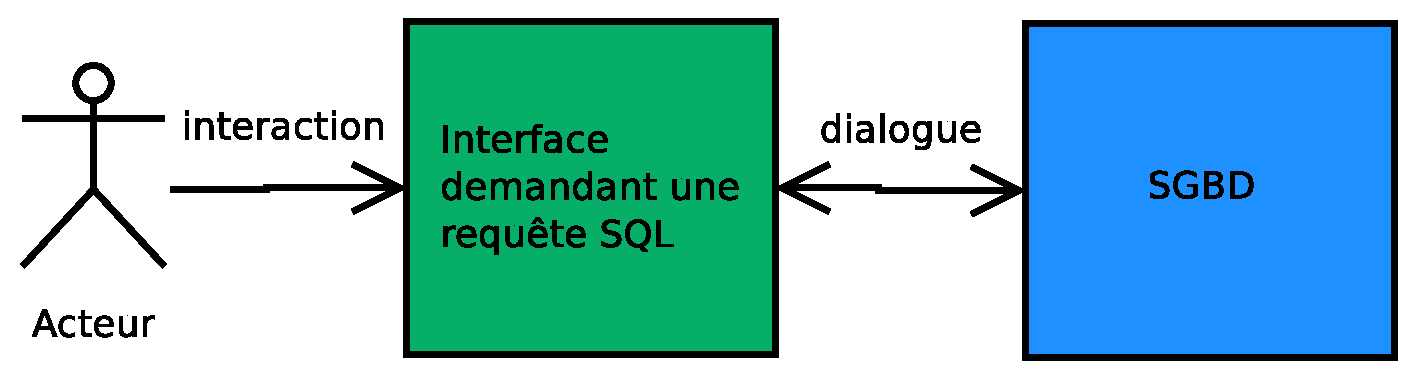
\includegraphics[width=14cm]{images/sans_idb.eps}
  \caption{Utilisation classique d'un SGBD.}
  \label{sans_idb_schema}
\end{figure}

\begin{figure}[!h]
  \centering
  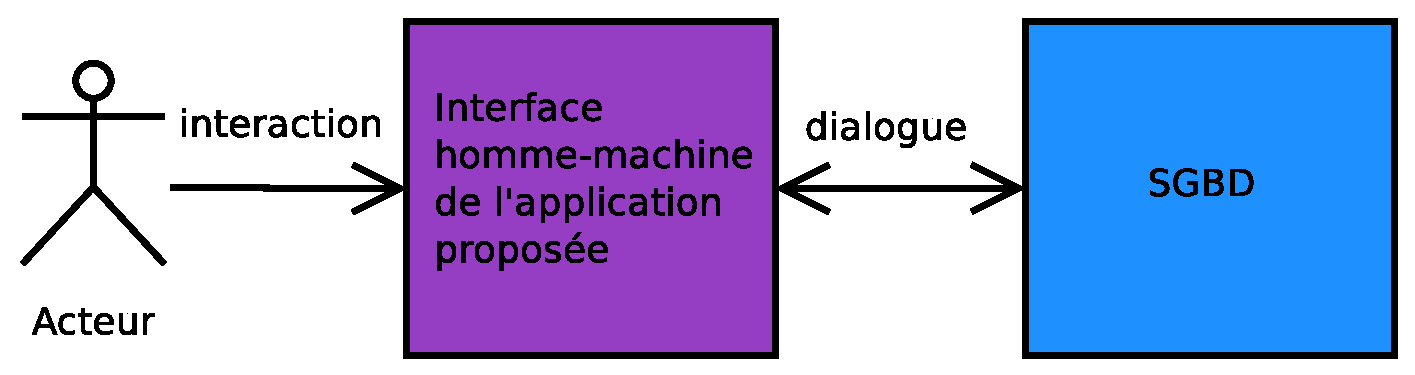
\includegraphics[width=14cm]{images/avec_idb.eps}
  \caption{Utilisation d'un SGBD avec l'application du projet.}
  \label{avec_idb_schema}
\end{figure}

\begin{figure}[!h]
  \centering
  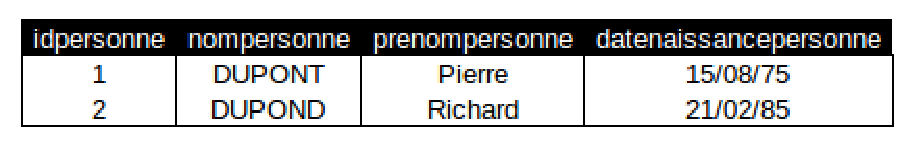
\includegraphics[width=14cm]{images/exemple_table.eps}
  \caption{Un exemple de table avec deux tuples et quatre attributs.}
  \label{exemple_table}
\end{figure}


\chapter{Analyse}
Comme mentionné précédemment, les SGBDR sont les plus utilisés des SGBD. Ils permettent de manipuler des bases de données relationnelles
par le biais du langage SQL. Puisque ce langage nécessite un certain apprentissage, un utilisateur ne le connaissant pas ne peut pas se servir
d'une base de données.

Ce projet tuteuré demande le développement d'une application permettant d'utiliser une base de données suivant deux directives :
\begin{itemize}
\item pas besoin d'utiliser le SQL,
\item compatible avec n'importe quel SGBD.
\end{itemize}

\section{Les fonctionnalités d'un SGBD}
L'application propose des fonctionnalités vues durant le cursus à l'IUT.

\subsection{Le \gls{ldd}}
Le langage de définition des données permet de structurer une base de données.
Il ne s'intêresse pas aux données contenues dans les tables
\footnote{\label{interet_ldd}Le LDD prend en compte les données contenues dans les tables et peut agir dessus, mais c'est une conséquence, pas son rôle.}, mais aux tables elles même. Le LDD est séparé en trois instructions:

\subsubsection{CREATE TABLE}
Permet de créer une \gls{table}. Dans un SGBD, les tables sont nommées, chaque nom est unique.
Une table est créée avec au moins un attribut dont il faut préciser le type de données (texte, nombre, date etc.) et la taille.
Des \glspl{constraint} supplémentaires peuvent être ajoutées, comme par exemple les \glspl{primarykey} \footnote{\label{contrainte_clée_primaire}Voir glossaire.}ou encore des \textit{NOT NULL}.

La \gls{query} suivante montre la création d'une table nommée PERSONNES, qui contient les attributs \textit{idpersonne}, \textit{nompersonne}, \textit{taillepersonne} et \textit{datenaissancepersonne}.

  \begin{lstlisting}
    CREATE TABLE PERSONNES
    (
    idpersonne CHAR(5),
    nompersonne VARCHAR(30),
    taillepersonne NUMBER,
    datenaissancepersonne DATE
    );
  \end{lstlisting}


\subsubsection{ALTER TABLE}
Permet de revenir sur ce qui a été fait avec CREATE TABLE.
L'instruction permet d'ajouter, supprimer ou modifier des \glspl{attribut}, des contraintes, des index...

Cette instruction se comporte différemment selon qu'une table soit vide ou remplie de lignes de données (\glspl{tuple}).
Par exemple, ajouter une contrainte NOT NULL sur une colonne possédant déjà des tuples nuls n'est pas possible. Ce problème n'existe pas sur une table vide.

La requête SQL suivante modifie la table \textit{PERSONNES} pour y ajouter une contrainte de clée primaire nommée \textit{pk\_personnes} sur l'attribut \textit{idpersonne}.

\begin{lstlisting}
  ALTER TABLE PERSONNES
  (
  ADD CONSTRAINT pk_personnes PRIMARY KEY (idpersonne)
  );
\end{lstlisting}

\subsubsection{DROP TABLE}
Permet de supprimer une table et les données qu'elle contient.
Dans une base de données relationnelles, les tables sont liées entre elles par des attributs.
La supression d'une table peut entraîner la supression de données dans d'autres tables, en fonction du schéma relationnel de la base.

La requête SQL suivante supprime la table \textit{PERSONNES} de la base de données.
\begin{lstlisting}
  DROP TABLE PERSONNES;
\end{lstlisting}

\subsection{Le \gls{lmd}}
Le langage de manipulation des données permet d'affectuer des actions de \gls{crud} sur ce que contiennent les tables.
En d'autres termes, il agit sur les tuples.

\subsubsection{Create}
Il d'agit de créer un nouveau tuple dans une table.
La requête SQL suivante permet d'ajouter un tuple de clée primaire \textit{00001} dans la table \textit{PERSONNES}.
\begin{lstlisting}
  INSERT INTO PERSONNES
  (idpersonne, nompersonne, taillepersonne,
  datenaissancepersonne)
  VALUES
  ('00001', 'DUPONT', 'Jean', '06/08/1985');
\end{lstlisting}

\subsubsection{Read}
Il s'agit de récupérer, lire, croiser des données que contiennent les tables.
Les requêtes SQL  "read" peuvent être très complexes.
Certains SGBD proposent des \glspl{qbe}
\footnote{Access, LOBase, phpMyAdmin...}pour créer ces requêtes sans manipuler de SQL.
Celle qui est écrite juste après est simple et permet de retrouver le nom de la \textit{PERSONNES} numéro "00001".
\begin{lstlisting}
  SELECT PERSONNES.nompersonne
  FROM PERSONNES
  WHERE PERSONNES.idpersonne = '00001';
\end{lstlisting}

\subsubsection{Update}
Il s'agit de modifier un ou plusieurs tuples qui existent déjà dans la base de données.
La requête SQL suivante remplace le nom de famille de la \textit{PERSONNES} "00001" par "Robert".
\begin{lstlisting}
  UPDATE PERSONNES
  SET nompersonne = 'Robert'
  WHERE idpersonne = '00001';
\end{lstlisting}

\subsubsection{DELETE}
Il s'agit de supprimer un ou plusieurs tuples.
La requête SQL suivante supprime les tuples des \textit{PERSONNES} qui s'appellent "Jean".
\begin{lstlisting}
  DELETE FROM PERSONNES
  WHERE prenompersonne = "Jean";
\end{lstlisting}

\subsection{Le Langage de Controle des Données (LCD)}
Cet aspect du SQL n'est pas demandé pour l'application et n'est pas traité.

\subsection{Transaction ACID}
Cet aspect des bases de données n'est pas demandé pour l'application et n'est pas traité.
En d'autres termes, une base de données ne peut être utilisée que par une seule personne à fois, sinon elle perd sa cohérence.

\section{Les IHM}
L'application fournie des IHM pour manipuler les bases de données sans utiliser le langage SQL.
Elle sont ergonomiques, non boguées et limitent les actions, empéchant de faire  erreurs.

L'application doit suivre les patterns habituels des applications posédant des vues.
L'utilisation des applications en couche ou du MVC est demandé.




\chapter{Conception}
Il nous a été nécessaire de créer des classes métiers représentant fidèlement le comportement réel des tables contenues dans n'importe quel \sgbd

\begin{figure}[!h]
\centering
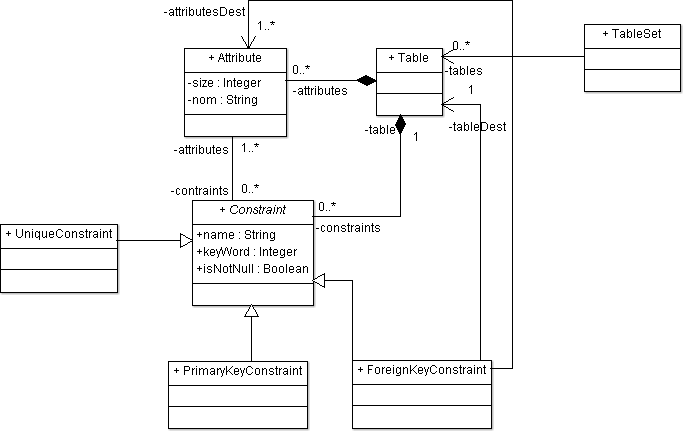
\includegraphics[width=18cm]{images/metier.png}
\caption{Diagramme de classes métiers}
\label{classes_metiers}
\end{figure}


Ces classes ont une particularité, elles peuvent générer du code SQL à partir de leurs attributs ou de différents arguments.
Lorsqu'une table est supprimé, tous les attributs de la table sont détruits et toutes les contraintes composant les attributs et la table sont détruit également.
Si un seul attribut est détruit, toutes les contraintes qui le compose sont détruites, ainsi, une contrainte \textbf{ForeignKeyConstraint} sera détruit même si elle concerne un second attribut.
\exemple{Une fk1 est composé de att1 et att2 pointant sur pk1 et pk2 respectivement.
\newline Si l'on supprime att1, alors la clé étrangère ne peut plus respecter la norme et la contrainte fk1 est détruite.}


\chapter{Manuel d'utilisation}
L'application se lance lors d'un double clique sur l'exécutable.

\section{Se connecter}
La première fen\^etre à apparaitre est l'interface de connexion ci-dessous :
\begin{figure}[!h]
\centering
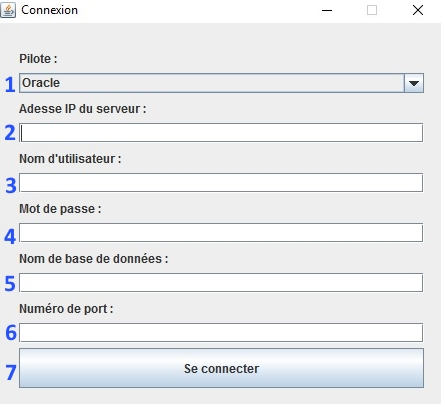
\includegraphics[width=10cm]{./images/manuel/se_connecter.jpg}
\caption{IHM - Se connecter}
\label{se_connecter}
\end{figure}

Afin de se connecter il faut renseigner les différents champs présents dans la fen\^etre.

\begin{enumerate}
\item choix du SGBD* (Oracle, MySQL).
\item Adresse IP du serveur ou est stockée votre base de données.
\item Nom d'utilisateur utilisé pour vous connecter à votre base de données. 
\item Mot de passe utilisé pour vous connecter à votre base de données.
\item Nom de la base de données.
\item Numéros de port du serveur ou est stockée votre base de données.
\item Cliquer sur le bouton \textbf{se connecter} pour tenter de se connecter au serveur.
\end{enumerate}

Connexion aux serveurs de l'IUT si vous \^etes étudiant :\\

\textbf{Oracle}
\begin{itemize}
\item SGBD : Oracle
\item Adresse IP : 162.38.222.149
\item Nom d'utilisateur : <nom-de-famille><première-lettre-du-prenom>
\item Mot de passe : <votre-INE>
\item Nom de la base de données : IUT
\item Numéros de port : 1521 \\
\end{itemize}

\textbf{MySQL}
\begin{itemize}
\item SGBD : MySQL
\item Adresse IP : 162.38.222.142
\item Nom d'utilisateur : <nom-de-famille><première-lettre-du-prenom>
\item Mot de passe : <votre-INE>
\item Nom de la base de données : <nom-de-famille><première-lettre-du-prenom>
\item Numéros de port : 3306
\end{itemize}

\section{Créer une table}
Dans le menu principal de l'application, cliquez sur le bouton \textbf{LDD : créer tables} pour ouvrir la fen\^etre de création de tables.

\begin{figure}[!h]
\centering
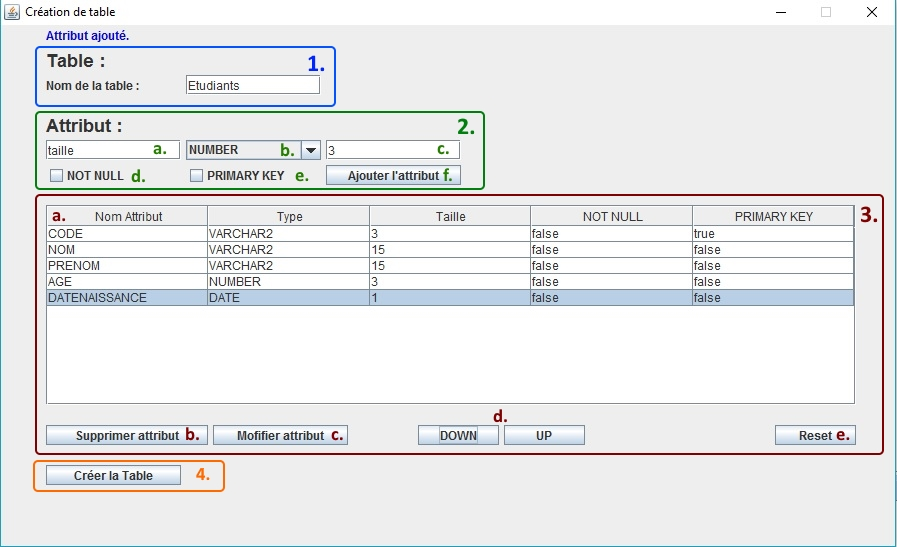
\includegraphics[width=14cm]{./images/manuel/creer_table.jpg}
\caption{IHM - Créer table}
\label{creer_table}
\end{figure}

\begin{enumerate}
\item Nom de ta table - \textit{ex : Etudiants}

\item Gestion des caractéristiques d'un attribut :
\begin{enumerate}
\item Nom - \textit{ex : codeEtudiant}
\item Type - \textit{ex : VARCHAR2}
\item Taille - \textit{ex : 15}
\item A cocher pour que l'attribut ne soit jamais null.
\item A cocher pour que l'attribut soit une clé primaire de votre table.
\item Cliquer sur le bouton \textbf{Ajouter l'attribut} pour tenter d'ajouter un attribut à la table.
\end{enumerate}

\item Gestion des attributs ajoutés :
\begin{enumerate}
\item Tableau contenant les attributs ajoutés avec le bouton <Ajouter l'attribut>.
\item Cliquer sur le bouton \textbf{Supprimer l'attribut} pour supprimer l'attribut sélectionné dans le tableau.
\item Cliquer sur le bouton \textbf{Modifier l'attribut} pour modifier l'attribut sélectionné dans le tableau. 
Les caractéristiques de l'attribut sélectionné sont à modifier dans la zone de gestion des caractéristiques d'un attribut. 
Vous pouvez ensuite valider ou annuler votre modification.
\item Cliquer sur les boutons \textbf{UP/DOWN} pour modifier l'odre des attributs dans le tableau. 
\item Cliquer sur le bouton \textbf{Reset} pour remettre à zéro la fen\^etre de création.
\end{enumerate}

\item Cliquer sur le bouton \textbf{Créer la table} pour tenter la création de la table.
\end{enumerate}

\section{Supprimer une table}
Dans le menu principal de l'application, cliquer sur le bouton \textbf{LDD : supprimer tables} pour ouvrir la fen\^etre de suppression de tables.

\begin{figure}[!h]
\centering
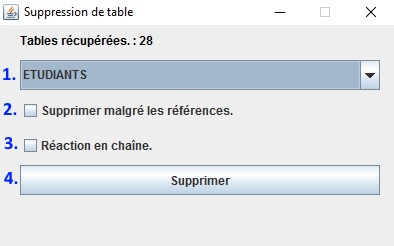
\includegraphics[width=8cm]{./images/manuel/supprimer_table.jpg}
\caption{IHM - Supprimer une table}
\label{supprimer_table}
\end{figure}

\begin{enumerate}
\item Choisir la table à supprimer.
\item A cocher pour supprimer sans prendre en compte les références des autres tables sur celle à supprimer.
\item A cocher pour supprimer la table sélectionnée puis toutes celles qui font référence à cette table et ceci récursivement.
\item Cliquer sur le bouton \textbf{Supprimer} pour tenter la suppression de la table.
\end{enumerate}

\section{Requ\^etes SQL}
Dans le menu principal de l'application, cliquer sur le bouton \textbf{SQL} pour ouvrir la fen\^etre du mode requ\^etes SQL.
\begin{figure}[!h]
\centering
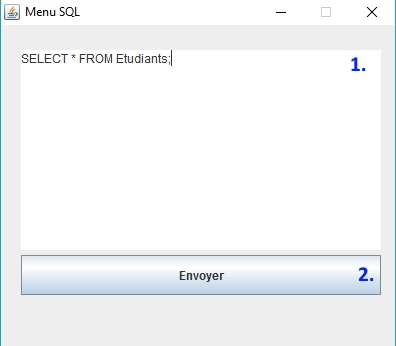
\includegraphics[width=6cm]{./images/manuel/sql.jpg}
\caption{IHM - SQL}
\label{sql}
\end{figure}

\begin{enumerate}
\item Ecrire la requ\^ete dans la zone de saisie - \textit{ex : SELECT * FROM Etudiants;} 
\item Cliquer sur le bouton \textbf{Envoyer} pour tenter d'exécuter la requ\^ete.
Une fenêtre s'ouvre indiquant le résultat de la requ\^ete si la syntaxe est correcte.
\end{enumerate}

\begin{figure}[!h]
\centering
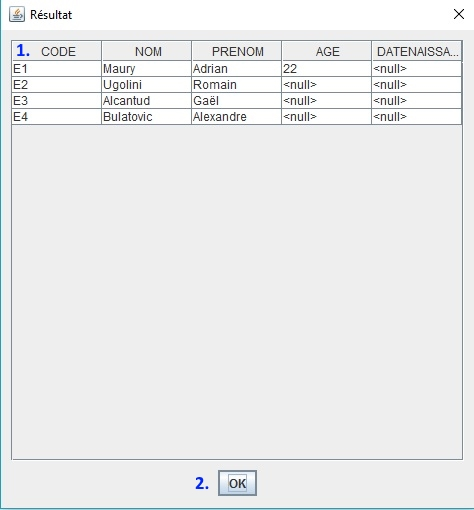
\includegraphics[width=8cm]{./images/manuel/sql_result.jpg}
\caption{IHM - Résultat SQL}
\label{sql_result}
\end{figure}

\begin{enumerate}
\item Résultat de la requ\^ete.
\item Cliquer sur le bouton \textbf{OK} pour fermer la fen\^tre de résultat.
\end{enumerate}

\section{CRUD* les tuples des tables}
Dans le menu principal de l'application, cliquer sur le bouton \textbf{CRUD} pour ouvrir la fen\^etre de gestion des tuples des tables.
\begin{figure}[!h]
\centering
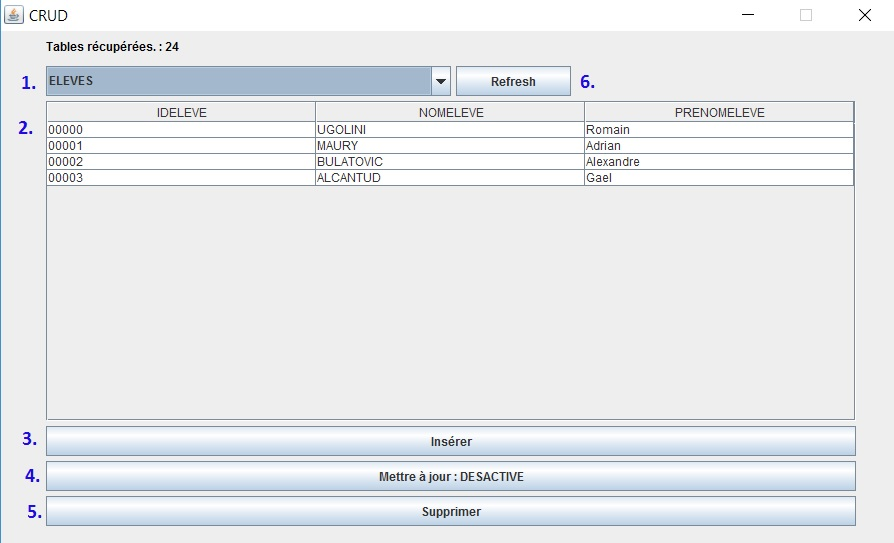
\includegraphics[width=12cm]{./images/manuel/crud.jpg}
\caption{IHM - CRUD}
\label{crud}
\end{figure}

\begin{enumerate}
\item Choisir la table.
\item Tableau contenant les différents tuples de la table sélectionnée.
\item Cliquer sur le bouton \textbf{Insérer} pour ajouter un tuple à la table. Il faut ensuite remplir les informations du nouveau tuple
dans la ligne vide qui s'est ajouté au tableau.
\item Cliquer sur le bouton \textbf{Mettre à jour} pour modifier un tuple de la table. Il faut ensuite modifer les informations du tableau et 
appuyer sur la touche entrée à chaque modification. Quitter le mode modification en cliquant une nouvelle fois sur le bouton \textbf{Mettre à jour}.
\item Cliquer sur le bouton \textbf{Supprimer} pour supprimer le tuple selectionné.
\end{enumerate}

\section{Ajouter et Supprimer des contraintes}


\backmatter

\end{document}
